\documentclass{article}
\usepackage{graphicx}
\usepackage[margin=1.5cm]{geometry}
\usepackage{amsmath}

\begin{document}
\twocolumn
\small

\title{Thursday Warm Up, Unit 2: Applications}
\author{Prof. Jordan C. Hanson}
\maketitle

\section{Memory Bank}

\begin{enumerate}
\item \textbf{Human audio range}, about 20 Hz - 20 kHz.
\item \textbf{Octave}, a factor of 2 in frequency.
\item \textbf{The volley principle}, frequency identification via rate of aural nerve signals.
\item \textbf{The place principle}, frequency identification via location of resonance on basilar membrane of the aural nerve within the cochlea.
\item \textbf{Decibels SPL} (sound power level). Logarithmic dB unit, where 0 dB SPL corresponds to $10^{-16}$ Watts cm$^2$.  This is about the minimum audible sound for human beings.  We can distinguish 1 dB SPL difference, and the loudest comfortable sounds have 120 dB SPL, so about 120 sound levels.
\item \textbf{Companding}, when digitization levels change non-linearly.
\item \textbf{Mu-law, for companding}.  To introduce the non-linearity necessary for logarithmically-spaced digital levels, the relationship between an input signal $x$ and an output signal $y$ is
\begin{equation}
y = \frac{\ln(1+\mu x)}{\ln(1+\mu)}
\end{equation}
with $\mu = 255$.
\end{enumerate}

\section{Audio Processing}

\begin{enumerate}
\item Suppose we are designing a music system, and must choose components that set the bandwidth and bits/sec of the sounds. (a) If the highest frequency we anticipate generating is 10 kHz, and we will digitize sounds with 16 bits per sample, how many bits/sec do we need to transmit? (b) If we cut our voltage resolution to 8 bits, how many bits/sec? (c) If we further reduce our max frequency to 3 kHz, while keeping 8 bits, how many bits/sec are required? \\ \vspace{2.5cm}
\item Suppose we're controlling volume with a knob, and at a certain knob setting, it gives 60 dB SPL of power. (a) What will the dB SPL be if we double the power by turning the knob? (b) If we use an amplifier and increase the power to 90 dB SPL, how would listeners react? (c) What is the ratio of power between 60 and 90 dB SPL? \\ \vspace{2.5cm}
\item Using the $\mu$-law, (a) calculate the difference $\Delta y = y_2 - y_1$ in signal outputs, given $x_2 = 10$ mV and $x_1 = 1$ mV.  Assume $\mu = 255$, and that all signals are in mV. (b) If we are using 8 bits, and our dynamic range is [1-256] mV, what is the \textit{linear} $\Delta V$ digitization? (c) How many digitization levels $\Delta V$ is $\Delta y$? (d) Repeat this process for $x_2 = 100$ mV and $x_1 = 1$ mV.
\end{enumerate}

\begin{figure}
\centering
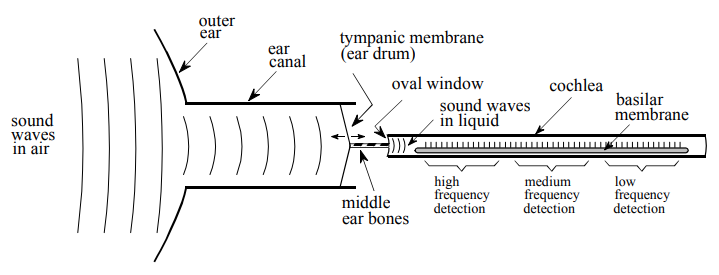
\includegraphics[width=0.4\textwidth]{audio_1.png}
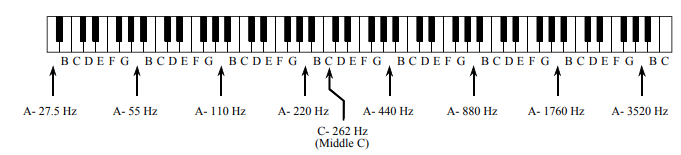
\includegraphics[width=0.4\textwidth]{audio_4.png}
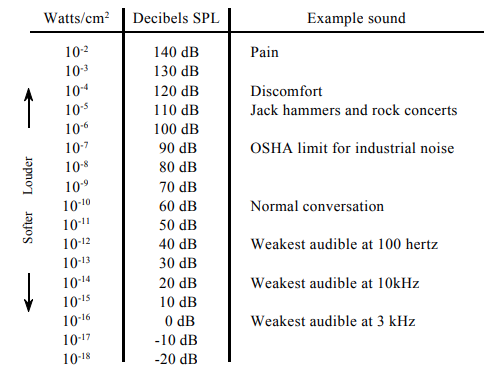
\includegraphics[width=0.4\textwidth]{audio_2.png}
\caption{\label{fig:1} (Top) Schematic of how the human ear works. (Middle) The piano keys cover most of the human hearing range, in a logarithmic sense.  One \textit{octave} is a factor of 2 change in frequency. (Bottom) dB SPL levels.}
\end{figure}

\end{document}
